\documentclass[../informe2.tex]{subfiles}
\begin{document}
%Que fue lo que se logró con la experimentación, incluir tablas y parámetros,
%gráficos, etc.\ lo más explicativo posible. Además destacar puntos
%importantes del problema, características de las instancias que influyeron
%en los resultados, valores de parámetros que influyeron en los resultados,
%análisis de calidad de las soluciones encontradas a través del tiempo,
%análisis en profundidad de la técnica vs los resultados obtenidos,
%valores promedio, desviaciones, \textbf{comparaciones con resultados de la literatura}, etc. También debería discutir qué cosas podría
%haber agregado o quedan como desafíos para trabajo futuro en su algoritmo.
\subsection{Greedy}
Como se detalló en la sección~\ref{sec:experimentos}, primero se verificó el funcionamiento del algoritmo \greedy, en relación a su efectividad en la creación de soluciones iniciales. Los resultados finales por cada instancia, se encuentran detallados en la tabla~\ref{tabla:greedy}.

\begin{table}[h]
	\small
	\makebox[\textwidth][c]{
	\begin{tabular}{@{}lrrrrrrrrrr@{}}
		\toprule
		Estadística/Instancia       & a1\_1 & a1\_2 & a1\_3 & a1\_4 & a1\_5 & a2\_1 & a2\_2 & a2\_3 & a2\_4 & a2\_5 \\ \midrule
		Total de procesos           & 100   & 1000  & 1000  & 1000  & 1000  & 1000  & 1000  & 1000  & 1000  & 1000  \\
		Procesos asignados          & 98    & 956   & 116   & 843   & 974   & 1000  & 945   & 4     & 62    & 58    \\
		\% de asignación    		& 98,00   & 95,60  & 11,60  & 84,30   & 97,40   & 100,00  & 94,50   & 0,40     & 6,20    & 5,80    \\
		Tiempo de ejecución [s] & 0     & 0     & 0     & 0     & 0     & 0     & 1     & 0     & 0     & 1     \\ %\bottomrule
	\end{tabular}}

	\makebox[\textwidth][c]{
	\begin{tabular}{@{}lrrrrrrrrrr@{}}
		\toprule
		& b\_1 & b\_2 & b\_3  & b\_4  & b\_5  & b\_6  & b\_7  & b\_8  & b\_9  & b\_10 \\ \midrule
		Total de procesos           & 5000 & 5000 & 20000 & 20000 & 40000 & 40000 & 40000 & 50000 & 50000 & 50000 \\
		Procesos asignados          & 2012 & 1962 & 14025 & 732   & 34082 & 13680 & 14050 & 44030 & 3609  & 3896  \\
		\% de asignación   	 		& 40,24 & 39,24 & 70,13 & 3,66   & 85,21 & 34,20 & 35,13 & 88,06 & 7,22  & 7,79  \\
		Tiempo de ejecución [s] & 2    & 2    & 8     & 26    & 22    & 26    & 300   & 29    & 117   & 300   \\ \bottomrule
	\end{tabular}}
	\caption{\small Por cada instancia, se muestra el número de procesos asignados con el algoritmo \textit{Greedy}.}\label{tabla:greedy}
\end{table}
\noindent En la tabla de arriba puede observarse la baja efectividad del algortimo \greedy\ en la generación de soluciones iniciales. Solamente en una instancia (a2\_1) se lograron asignar todos los procesos (mil en total). En esta, se consiguió un costo total de 224150350, más bajo que los
391189190 de la solución inicial provista en el desafío de la \roadef. En términos generales puede observarse que:
\begin{itemize}
	\item Se observa una mayor tasa de asignación en las instancias donde hay un alto grado de servicios sin dependencias y \textit{spreadmin} de cero. De hecho la instancia (a2\_1), todos los servicios cumplen con esas características.
	\item En la mayoría de las instancias, los procesos asignados son solamente los que pertenecen al conjunto $\mathcal{LRP}$. Para cada instancia del dataset b, el número de procesos asignados coincide con el número de servicios sin dependencias y \textit{spreadmin} de cero (comparar con cuadro~\ref{tabla:analisis-servicios}). Esto indica que esos servicios son mono-proceso. Solamente la primera parte del \greedy\ gozó de efectividad.
	\item Las instancias a1\_1 y a2\_2 no poseen dependencias (ver cuadro~\ref{tabla:set-a}). La causa de no poder asignar todos los procesos, se debe a problemas de capacidad disponible en las máquinas respectivas. Esto indica que los procesos están mal distribuidos, considerando que con los mismos procesos y máquinas, en el desafío de la \roadef\ se provee una solución inicial factible. En ese sentido sentido, la función miope no es efectiva ni eficiente. En relación a esto último, el éxito logrado en (a2\_1) se debió al asignar, los procesos de $\mathcal{LRP}$ con un mayor tamaño primero (suma de todos sus requerimientos). A pesar de ser el funcionamiento por defecto de la primera parte del \greedy, no se obtuvieron otros resultados satisfactorios.
	\item Puede evidenciarse que la segunda parte del algoritmo \greedy\ tuvo una efectividad practicamente nula, a excepción de unas cuantas instancias de los datasets a1 y a2. En esa parte del algoritmo, en comparación con la primera, se chequean además las restricciones de dispersión y dependencia. Durante el desarrollo de la aplicación se mostró que la restricción de dependencia era la que se violaba de forma constante, no pudiendo realizar más asignaciones. Lo anterior puede explicarse porque los servicios pertenecientes al conjunto $\mathcal{RS}$, no dependen de los servicios asignados en la primera parte del \greedy\ ($\mathcal{LRS}$). Más bien, las redes de dependencias se encuentran cerradas en $\mathcal{RS}$, es decir, un servicio $s_a \in \mathcal{RS}$, solamente depende de otros que pertencen al mismo conjunto. La situación se complejiza cuando se tienen dependencias circulares, en que $s_a$ depende de $s_b$ y viceversa, arrojando la interrogante de por dónde comenzar a asignar sin tener que violar las restricciones de dependencia.
	\item Importante es señalar que el análisis previo realizado sobre las características de los servicios, en torno al mínimo de dispersión y de cantidad de dependencias, puede resultar demasiado específico en función de las instancias utilizadas para realizar las distintas pruebas presentadas en este informe. Las instancias son generadas de forma aleatoria y nada asegura que la mayoría de los servicios generados posean las características antes mencionadas.
\end{itemize}
\noindent Tomando en consideración el análisis anterior y la baja efectividad en el propósito buscado, la implementación de un algoritmo \greedy\ es bastante compleja e innecesaria, para el solo hecho de generar una solución factible. Si a esto se suma además que el \mrp\ por definición, considera la provisión de una solución inicial factible, intentar generar otra es un gasto no deseable de recursos (tiempo especialmente). Finalmente, el hecho de que en la literatura no se haga mención de una estrategia similar, es una prueba más de que es más conveniente comenzar mejorando la solución que se provee inicialmente por defecto.

\subsection{Hill Climbing}
A diferencia del algorimo \greedy, el \hillc\ \textit{mejor mejora} mostró resultados efectivos y en algunos casos bastante buenos, considerando la simplicidad del mismo. Se testearon dos modalidades del \hillc, con formas distintas de seleccionar los procesos para generar las vecindarios: HC, selección según secuencia de lectura instancia; y HC-SP (\hillc\ \textit{sorted processes}), selección según tamaño de los procesos (descendentemente). Los resultados finales de las pruebas se encuentran en detalle en el cuadro~\ref{tabla:hc-comparative}. Ahí puede verse que ambas modalidades del \hillc\  logran disminuir el costo total, mejorando la solución inicial. El número de iteraciones (en el pseudocódigo~\ref{algorithm:HC}, son las veces en que se intenta generar un nuevo vecindario) es similar en ambas modalidades, a excepción de la b\_5. En ambos casos, los tiempos de ejecución se mantienen por debajo del medio minuto hasta la instancia b\_1 y debajo del tiempo límite hasta la b\_3, por lo que puede decirse que los algoritmos terminan cuando ya no hay más reasignaciones posibles que realizar. A partir de la instancia b\_4, los tiempos de ejecución llegan a los 300[s], por lo que el tiempo límite es la condición de parada que se activa. Comparando entre sí ambos métodos en función del costo total, se tiene que la versión HC-SP logra mejores resultados en 14 de las 20 instancias probadas (ver columna Diferencia), resultado que es bastante notorio en las últimas cuatro instancias (ver también figura~\ref{fig:comparativa-hc}). Esto es concordante por lo expresado por Gavranović et.al~\cite{gavranovicefficient}, donde reasignar los procesos más grandes primero, permite generar mejores resultados.
\makeatletter
\setlength{\@fptop}{0pt}
\makeatother
\begin{table}[ht!]
	\footnotesize
	\makebox[\textwidth][c]{
\begin{tabular}{@{}lrrrrrrrr@{}}
\toprule
Instancia & Inicial & HC & Tiempo & Iteraciones & HC-SP & Tiempo & Iteraciones & Diferencia \\ \midrule
a1\_1     & 49528750                    & 44307612               & 0                          & 200                             & 44306501                  & 0                          & 200                             & -1111                          \\
a1\_2     & 1061649570                  & 878229613              & 1                          & 3000                            & 929137945                 & 0                          & 2000                            & 50908332                       \\
a1\_3     & 583662270                   & 583384296              & 1                          & 3000                            & 583373392                 & 1                          & 2000                            & -10904                         \\
a1\_4     & 632499600                   & 570401602              & 0                          & 2000                            & 568344744                 & 0                          & 2000                            & -2056858                       \\
a1\_5     & 782189690                   & 728145497              & 1                          & 4000                            & 737253098                 & 1                          & 3000                            & 9107601                        \\
a2\_1     & 391189190                   & 35481989               & 4                          & 7000                            & 38489889                  & 4                          & 5000                            & 3007900                        \\
a2\_2     & 1876768120                  & 1494274528             & 2                          & 7000                            & 1415300243                & 0                          & 3000                            & -78974285                      \\
a2\_3     & 2272487840                  & 1869593233             & 1                          & 5000                            & 1734732392                & 1                          & 3000                            & -134860841                     \\
a2\_4     & 3223516130                  & 2283923795             & 3                          & 9000                            & 2128654638                & 3                          & 8000                            & -155269157                     \\
a2\_5     & 787355300                   & 650311032              & 2                          & 9000                            & 612089208                 & 2                          & 8000                            & -38221824                      \\
b\_1      & 7644173180                  & 5271411947             & 10                         & 20000                           & 5314076290                & 7                          & 15000                           & 42664343                       \\
b\_2      & 5181493830                  & 1278123023             & 91                         & 60000                           & 1150616078                & 110                        & 70000                           & -127506945                     \\
b\_3      & 6336834660                  & 1149013744             & 248                        & 180000                          & 1953270617                & 64                         & 80000                           & 804256873                      \\
b\_4      & 9209576380                  & 4679312094             & 300                        & 30489                           & 4678242633                & 300                        & 30887                           & -1069461                       \\
b\_5      & 12426813010                 & 2968606165             & 300                        & 48269                           & 3252021891                & 298                        & 200000                          & 283415726                      \\
b\_6      & 12749861240                 & 9526211153             & 300                        & 42377                           & 9526194551                & 300                        & 43333                           & -16602                         \\
b\_7      & 37946901700                 & 31761671090            & 300                        & 4872                            & 18067048987               & 300                        & 10248                           & -13694622103                   \\
b\_8      & 14068207250                 & 6651200779             & 300                        & 21484                           & 5314963613                & 300                        & 95278                           & -1336237166                    \\
b\_9      & 23234641520                 & 16030720890            & 300                        & 9337                            & 15896062116               & 300                        & 17959                           & -134658774                     \\
b\_10     & 42220868760                 & 38023415516            & 300                        & 3620                            & 20990879440               & 300                        & 9822                            & -17032536076                   \\ \bottomrule
\end{tabular}}
\caption{\small Detalle de los resultados obtenidos, utilizando las dos versiones del algoritmo \textit{Hill Climbing}.}\label{tabla:hc-comparative}
\end{table}

\begin{figure}[ht!]
	\makebox[\textwidth][c]{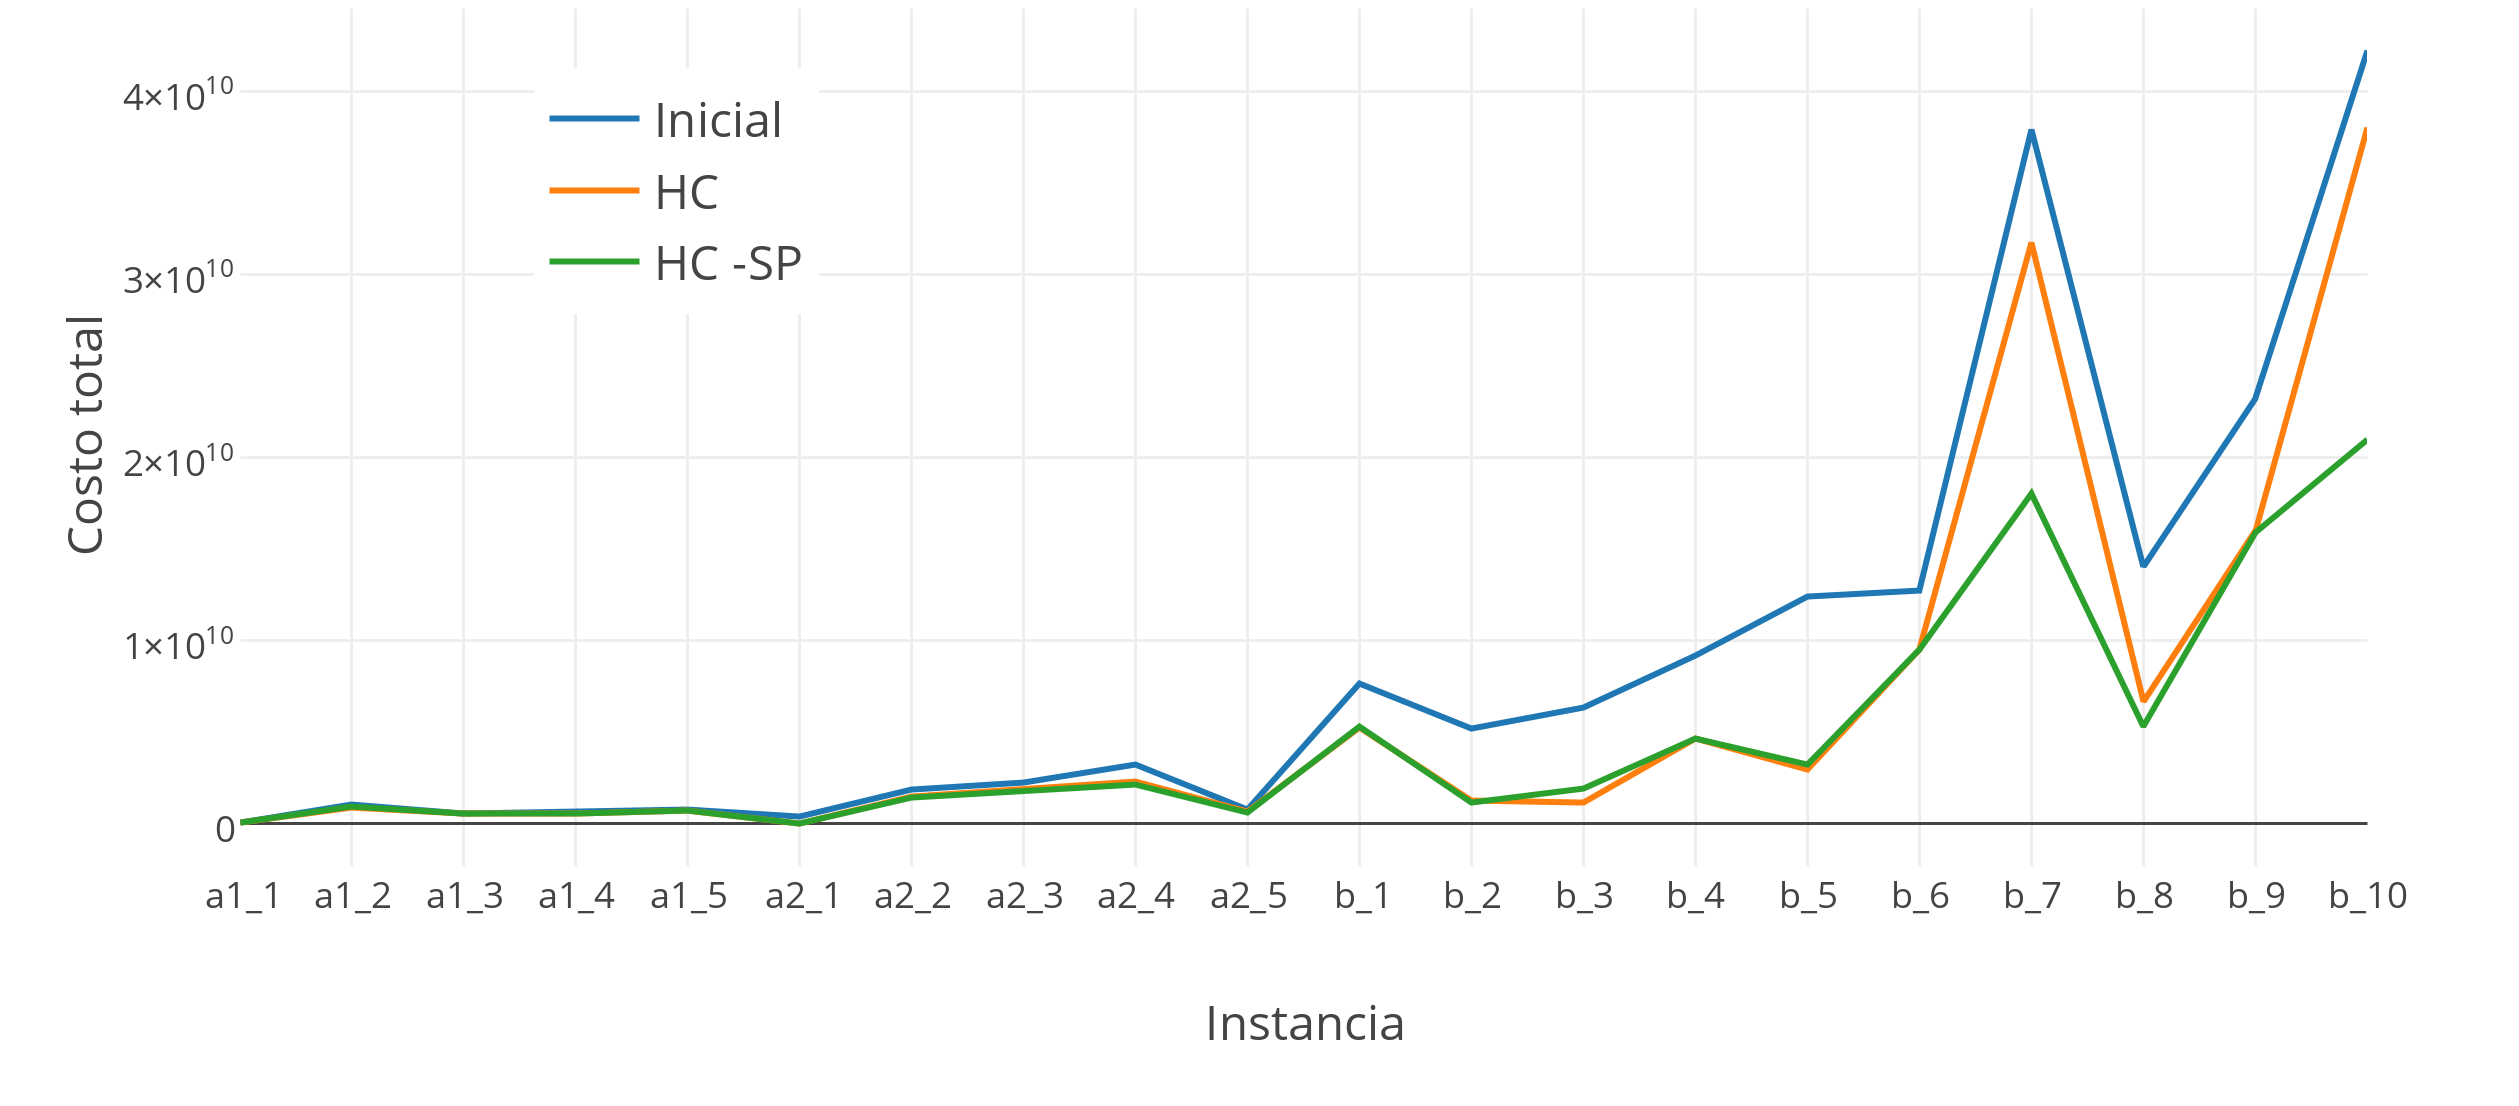
\includegraphics[width=1.1\textwidth]{comparativa-hc.png}}
	\caption{\small Costo total inicial y los resultados entregados las dos versiones del \hillc.}\label{fig:comparativa-hc}
\end{figure}

\noindent Determinada la mejor versión del \hillc, ahora se compara con los mejores resultados obtenidos en la \roadef. El detalle puede encontrarse en el cuadro~\ref{tabla:comparative-with-best-roadef}. Puede verse que el HC-SP obtiene resultados inferiores en todas las instancias. Sin embargo, puede decirse que en las instancias a1\_1, a1\_3, a1\_5, b\_2, b\_4, b\_4, b\_9 y b\_10, está dentro del orden de magnitud del mejor (ver también figura~\ref{fig:comparativa-hc-best-challenge}), por lo que el \hillc\ \textit{mejor mejora}, genera resultados para nada despreciables, considerando la heurística simple en la cual está basado. En relación a implementaciones alternativas, la generación de vecindarios podría generarse no en función de un \textit{shift}, sino que en función de un movimiento de \textit{swap}. Este involucra el intercambio de la asignación de dos procesos, originalmente asignados a dos máquinas distintas. Con un \textit{shift}, el tamaño de los vecindarios originados es $O(|\mathcal{P}|\times|\mathcal{M}|)$. Para un \textit{swap} el tamaño del vecindario es $O(|\mathcal{P}|^{2})$. Considerando que comúnmente, la cantidad de procesos es mucho mayor que el número de máquinas, utilizar un \textit{swap} como movimiento hace que se obtengan una mayor cantidad de soluciones vecinas, por lo que sería posible mejorar en mayor medida el costo total.

\begin{table}[h]
	\small
\centering
\begin{tabular}{@{}lrrr@{}}
\toprule
Instancia & Inicial & Mejor ROADEF 2012 & HC-SP \\ \midrule
a1\_1  & 49528750               & 44306501            & 44306501              \\
a1\_2  & 1061649570             & 777532896           & 929137945             \\
a1\_3  & 583662270              & 583005717           & 583373392             \\
a1\_4  & 632499600              & 252728589           & 568344744             \\
a1\_5  & 782189690              & 727578309           & 737253098             \\
a2\_1  & 391189190              & 198                 & 38489889              \\
a2\_2  & 1876768120             & 816523983           & 1415300243            \\
a2\_3  & 2272487840             & 1306868761          & 1734732392            \\
a2\_4  & 3223516130             & 1681353943          & 2128654638            \\
a2\_5  & 787355300              & 336170182           & 612089208             \\
b\_1   & 7644173180             & 3339186879          & 5314076290            \\
b\_2   & 5181493830             & 1015553800          & 1150616078            \\
b\_3   & 6336834660             & 156835787           & 1953270617            \\
b\_4   & 9209576380             & 4677823040          & 4678242633            \\
b\_5   & 12426813010            & 923092380           & 3252021891            \\
b\_6   & 12749861240            & 9525857752          & 9526194551            \\
b\_7   & 37946901700            & 14835149752         & 18067048987           \\
b\_8   & 14068207250            & 1214458817          & 5314963613            \\
b\_9   & 23234641520            & 15885486698         & 15896062116           \\
b\_10  & 42220868760            & 18048515118         & 20990879440           \\ \bottomrule
\end{tabular}
\caption{\small Mejor resultado obtenido en el desafío de la \roadef\ y el conseguido con \textit{HC-SP}.}\label{tabla:comparative-with-best-roadef}
\end{table}
\begin{figure}[h]
	\makebox[\textwidth][c]{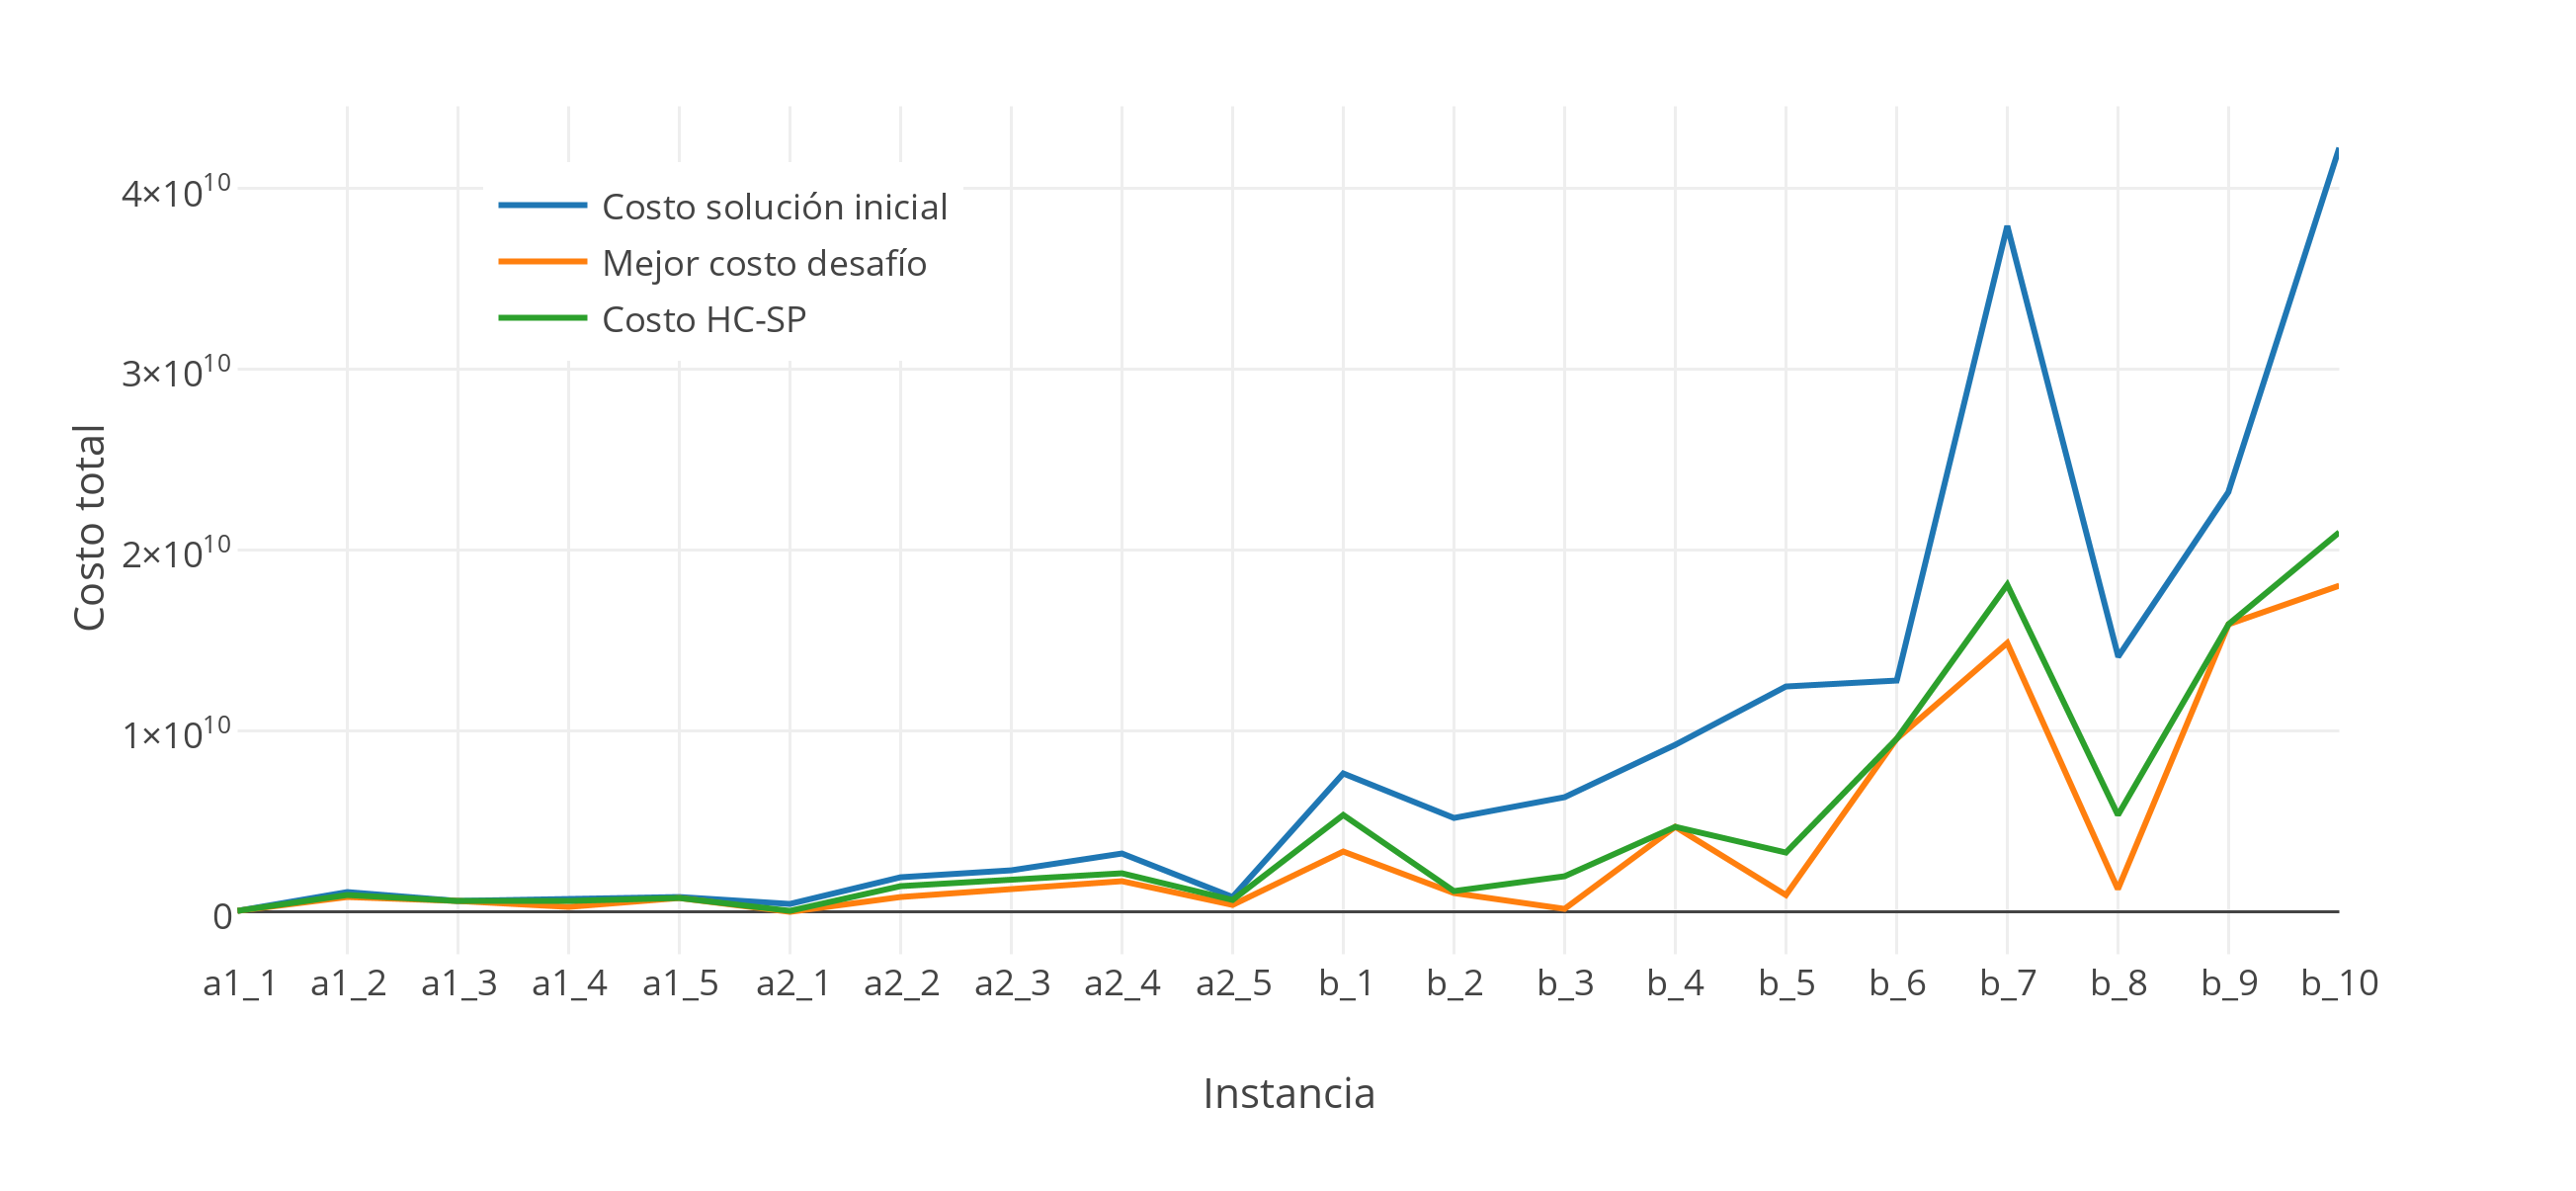
\includegraphics[width=1.1\textwidth]{comparativa-hc-best-challenge.png}}
	\caption{\small Costo total inicial, mejor resultado en la \roadef\ y del \hillc\ \textit{sorted processes}.}\label{fig:comparativa-hc-best-challenge}
\end{figure}
\clearpage

\end{document}
